\documentclass{article}

% ready for submission: preprint or final
\usepackage[preprint]{neurips_2023}


\usepackage[utf8]{inputenc} % allow utf-8 input
\usepackage[T1]{fontenc}    % use 8-bit T1 fonts
\usepackage{hyperref}       % hyperlinks
\usepackage{url}            % simple URL typesetting
\usepackage{booktabs}       % professional-quality tables
\usepackage{amsfonts}       % blackboard math symbols
\usepackage{nicefrac}       % compact symbols for 1/2, etc.
\usepackage{microtype}      % microtypography
\usepackage{xcolor}         % colors
\usepackage{graphicx}


\title{Gaussian Evolution Strategies}

\author{%
  Bram Pulles\\
  Department of Artificial Intelligence\\
  Radboud University\\
  \texttt{S1015194}\\
  \texttt{bram.pulles@ru.nl} \\
}


\begin{document}


\maketitle


\begin{abstract}
	The inverted pendulum problem is a widely known simple environment in which
	different machine learning approaches are tested. We compare the
	performance of the reinforce algorithm and a simple Gaussian evolutionary
	strategy (ES) for solving the inverted pendulum problem. We rely heavily on
	hardware acceleration using JAX and show that the ES implementation
	performs a magnitude faster than the reinforce implementation. We conclude
	that the ES is a promising approach with good convergence properties for
	this particular problem.
\end{abstract}


\section{Introduction}
\label{sec: introduction}
Reinforcement learning (RL) consitutes a broad field of machine learning
methods in which agents are trained by rewarding desirable behaviours and
punishing undesirable behaviours. We aim to teach an agent how to solve the
inverted pendulum problem. In this problem the agent guides the bob (the object
on the pendulum) to the unstable fixed point at the top of the pendulum, see
figure \ref{fig: inverted pendulum}. Using RL methods the agent can be trained
to show this desired behaviour.

\begin{figure}[h]
	\centering
	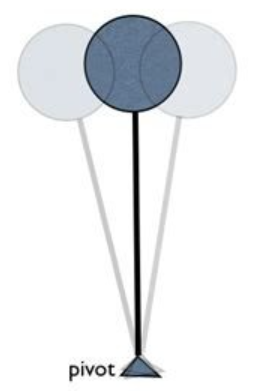
\includegraphics[width = 0.2\textwidth]{images/inverted_pendulum.png}
	\caption{Pendulum with the bob at the unstable fixed point.}
	\label{fig: inverted pendulum}
\end{figure}

We have previously shown how the reinforce algorithm, also known as the Monte
Carlo policy gradient algorithm, can be utilized to teach the agent how to
solve the inverted pendulum problem.\footnote{This was done in assignment 8. We
use the provided solution as reference implementation.} This method is based on
the idea of using gradient descent to optimize a policy by directly optimizing
the cumulative reward. Instead of using a gradient-based RL method, we contrast
the approach with a gradient-free simple Gaussian evolution strategy.

Evolutionary strategies (ES) and gradient-based approaches are two different
families of optimization methods each with their own strengths and weaknesses.
Here are some reasons why ES might be preferred over gradient-based approaches:

\begin{itemize}
	\item
		ES can perform well in stochastic environments. Since ES samples
		solutions from a distribution it is flexible and can adapt to uncertain
		environments better than gradient-based methods which might get stuck
		in a local solution space due to the noise. In general, ES tend to
		explore the search space more globally than gradient-based methods due
		to this property.
	\item
		ES can be applied to problems where gradients may not be available or
		expensive to compute. This includes problems with discontinuous and
		non-differentiable objective functions. It would be challenging to use
		gradient-based methods for solving such problems.
	\item
		ES are easy to parallelize. ES can exploit distributed hardware or
		other parallel computing power. This way, the performance, or cumulative
		reward in our case, of various solutions can be computed
		simultaneously. This can lead to faster convergence times, especially
		when taken advantage of hardware capabilities with a library like JAX.
\end{itemize}

It is clear now why ES are interesting when contrasted to other gradient-based
approaches. In section~\ref{sec: methods} we define a research question and
outline the ES that we implement to solve the inverted pendulum problem. In
section~\ref{sec: results} we discuss the performance of the ES and compare
this to the previously implemented reinforce algorithm. We end with a
discussion of the results in section~\ref{sec: discussion}.

\section{Methods}
\label{sec: methods}

\subsection{Research question}
\label{sec: research question}
In line with the introductory goals, we aim to train an agent for solving the
inverted pendulum problem. To this end we use the pendulum implementation from
Gym, a toolkit for developing and comparing reinforcement learning algorithms
made by OpenAI. We implement a straightforward Gaussian evolutionary strategy.
For both the ES and the reinforce algorithm we aim to answer the following
question:

\begin{quote}
	How does the simple Gaussian ES perform compared to the reinforce algorithm
	in terms of convergence, measured in time and in number of iterations
	needed?
\end{quote}

By considering the runtime, we benchmark the training duration for each
algorithm. Additionally, the number of iterations needed by either algorithm to
converge provides another metric giving an impression of the performance. We
expect that the ES will converge faster compared to the reinforce algorithm,
due to the high cost of calculating the cumulative reward for the objective
function and the parallelisability of the ES. For the implementation we use JAX
which can make good use of the available concurrency capable hardware.

\subsection{Evolutionary strategy}
\label{sec: evolutionary strategy}
The agents that we use for both the reinforce algorithm and the ES consist of a
simple neural network with one hidden layer. The network is supposed to apply a
force to the bob such that the bob is balance in the unstable fixed point. To
this end it gets information at every time step. As input it gets the $(x, y)$
position and the angular velocity of the bob. As output it gives a probability
distribution over three possible actions: -1, 0 or 1 torque applied to the free
end of the pendulum. The agents performance is measured by computing the mean
cumulative reward across multiple rollouts.

The neural network completely defines the agent. Let all the parameters, i.e.
the weights and biases for each layer, be defined in one long vector
$\overline\theta$. Our goal is to find an optimal $\overline\theta$ such that
the inverted pendulum problem is solved by the neural network defined as
$\overline\theta$.

In order to do this using the evolutionary strategy we start with creating a
$n$-dimensional Gaussian distribution $p_\theta \sim \mathcal{N}(\overline\mu,
\overline\sigma^2 I)$ with $\overline\mu$ as the best estimate for each
parameter of $\overline\theta$ and $\overline\sigma$ the uncertainty for each
parameter. The function $p_\theta$ can be initialized with some vector
$\overline\mu$ and $\overline\sigma$.

Next, we generate a population of $N$ sample neural networks $D$ from
$p_\theta$. This can be seen as the offspring from the current best estimate of
$\theta = \overline\mu$ modelled in $p_\theta$. For all the networks in $D$ we
compute the mean cumulative reward across multiple rollouts, giving us a
performance score for each network in the population. We select the top $k < N$
performing sample networks and call this the elite set $D_\mathtt{elite}
\subset D$. Now we estimate the new variance as the squared difference between
all samples in the elite set and the previous mean $\overline\sigma =
\frac{1}{N} \sum^k_{i=1} \left( \overline\theta_i - \overline\mu \right)^2$ .
The new mean $\overline\mu$ is computed by taking the mean over all $\theta_i
\in D_\mathtt{elite}$. This leaves us with a new and hopefully better
$p_\theta$. We now throw away the old $D$ and repeat these steps until $\theta
= \overline\mu$ is satisfactory.

\section{Results}
\label{sec: results}
The results for the training session of the reinforce algorithm are shown in
figure \ref{fig: reinforce}. We use the provided hyperparameter settings: 64
hidden nodes, a learning rate of 0.005, gamma (the reward discount factor) is
0.99, the number of batches is 50 and the number of steps per episode is 200.
The first time running this takes 82.6 seconds. Running it for the second time,
which is faster because JAX does not need to compile again, takes 78.8 seconds.

The results for the training session of the Gaussian ES are shown in figure
\ref{fig: ES}. The hyperparameter settings used are as follows: 10 hidden
nodes, gamma is 0.99, the number of steps per episode is 200, we use 50
rollouts per sample to measure the performance, the population size $N$ is 100
and we select the top $k = 10$ best performing networks, we start with
$\overline\mu = \overline0$ (all zeros) and $\overline\sigma = \overline{100}
I$ (a matrix with 100's on the diagonal). The first time running takes a mere
4.6 seconds and a second time only 3.1 seconds.

Given these results we can already conclude that the ES implementation is
time wise a whole magnitude faster than the reinforce implementation. We also
see that it takes only about 50 iterations to converge, compared to about 2000
iterations needed for the reinforce algorithm. Interestingly, when the ES
implementation is run without being compiled through JAX, it takes over an hour
to run, so JAX greatly decreases the runtime. We also found that for the
Gaussian ES the choice of the initial $\overline\sigma$ matters a lot, if this
is chosen to small the algorithm does not converge to a solution. The other
hyperparameters have less influence on the training trajectory.

\begin{figure}[h]
	\centering
	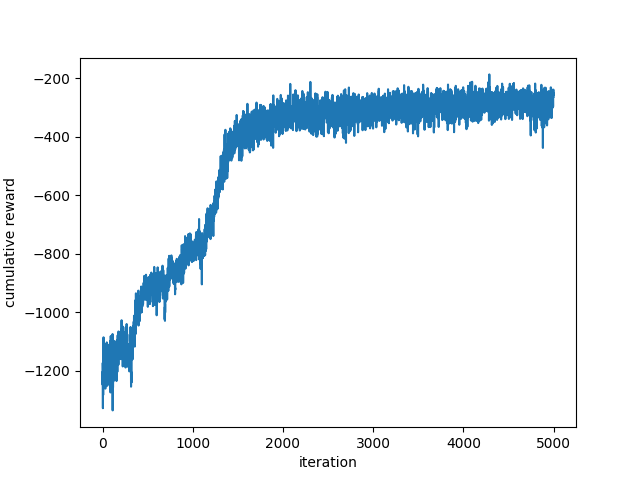
\includegraphics[width = 0.7\textwidth]{images/reinforce.png}
	\caption{Reinforce algorithm training results.}
	\label{fig: reinforce}
\end{figure}

\begin{figure}[h]
	\centering
	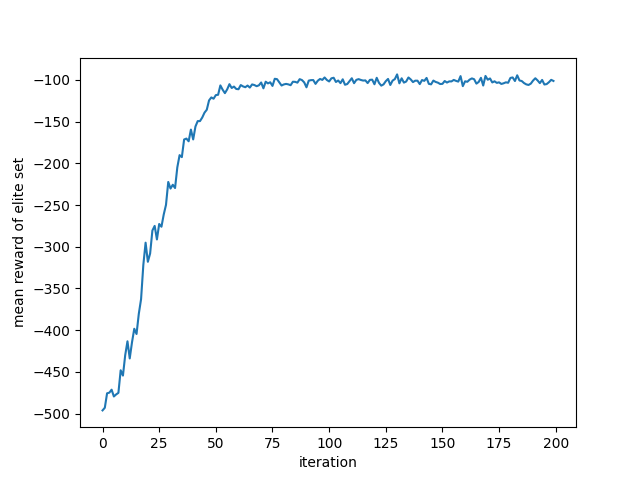
\includegraphics[width = 0.7\textwidth]{images/ES.png}
	\caption{Gaussian evolutionary strategy training results.}
	\label{fig: ES}
\end{figure}

\section{Discussion}
\label{sec: discussion}
The results show a clear victory for the Gaussian ES compared to the reinforce
algorithm, however there are a lot of side notes that should be placed here.
First, we did not do any hyperparameter search. For the ES we have done this
manually, while for the reinforce method we just took the given parameters. In
order to do a fairer comparison a hyperparameter search is needed. Second, the
reinforce implementation can likely be sped up more using JAX. For example, a
forward pass through the network is not compiled now, while it is for ES
method. Working more on the implementation details particularly with speed in
mind can therefore improve the performance of both algorithms, but especially
for the reinforce version. Third, the ES implementation can make good use of
parallel hardware available in the computer used to run the training. If this
would not be available the time performance of the ES would probably be a lot
worse, since it heavily relies on parallelisation for computing a lot of
forward passes through all the networks simultaneously.

While benchmarking the Gaussian ES there were quite some difficulties with
finding the right hyperparameter settings. In particular because the importance
of $\overline\sigma$ was overseen. There are two ways to tackle this problem.
One is the already mentioned parameter search, this would likely find out that
the value for $\overline\sigma$ is very important. Another solution would be to
alter the ES currently used. As it is implemented now the variance depends
heavily on the previous parameters of $\overline\mu$. An alternative method
which aims to address to problems is the covariance matrix adaptation ES
(CMA-ES). This algorithm could be implemented instead, but greatly increases
the complexity.

Another important aspect of the analysis done is the problem that was chosen.
In our case we tackled the inverted pendulum problem. For this problem the ES
performed quite well. It would be interesting to expand the number of problems
and compare against multiple problems to give a better comparison between the
two methods.

All in all, the Gaussian evolutionary strategy gave us promising results.
However, a more elaborate research is definitely required to provide us with a
comparison that is trustworthy and representative of the performance
differences between the Gaussian ES and the reinforce algorithm.


\section*{Acknowledgements}
The simple Gaussian evolutionary strategy approach is taken from Lilian Weng's
blog.\footnote{\url{https://lilianweng.github.io/posts/2019-09-05-evolution-strategies/}}
The alternative method of CMA-ES was also found here. We also used the solution
provided for assignment 8 and of course the syllabus written for the course.
Lastly, we heavily relied on JAX in order to create a speedy implementation for
both the algorithms.

\end{document}
